\section{Durchführung}
    \subsection{Reaktorstart}
    \underline{\textbf{Vor Inbetriebnahme}}  \\ 
    Vor der Inbetriebnahme des Reaktors sind mehrere sicherheitsrelevante Prüfungen an dosimetrischen und nicht-dosimetrischen Einrichtungen vorzunehmen. Zu Beginn werden insbesondere die Anzeigen und Warnsignale auf ihre Funktionalität überprüft, da sie auf Grenzwertüberschreitungen und eine mögliche Reaktorschnellabschaltung hinweisen sollen. Nicht zuletzt wird darüber auch gewährleistet, dass die Messgeräte Signale geben,um als Reaktion darauf eine eventuelle Abschaltung des Reaktors zu verhindern.\\
    Eine RESA findet unter verschiedenen Umständen statt. Zum einen ereignet sie sich bei einer Leistung von weniger als 0,25\unit{W}, da die Neutronenzählrate direkt Proportional zur Leistung sein soll, die statistischen Fehler allerdings bei geringen Leistungen zu groß werden. Einen Warnton erhält man bei 0,3\unit{W}. Zum anderen erfolgt eine RESA durch bei überhöhte Leistung bei 2,4\unit{W}. Einen Warnton erhält man ab 2,2\unit{W}.
    Als Abschaltgrund gilt auch eine zu geringe Reaktorperiode. Während des Versuchs ist als Richtwert eine untere Grenze von 30\unit{s} einzuhalten. Eine Warnung ertönt bei 20\unit{s}, die RESA erfolgt bei 10\unit{s}.
    Ein weiterer Grund für die RESA stellt die Temperatur des Moderators dar. Unterschreitet dieser 22\unit{°C} erfolgt hier eine Abschaltung.\\ \ \\
    \underline{\textbf{Start}}\\
    Ist man sich dieser Grenzwerte bewusst und hat man das akustische Signal gehört, kann fortgefahren werden. Man fährt die Anfahrneutronenquelle ein (ANQ) und beobachtet Änderungen in Leistung und Impulsraten (siehe Tablle \ref{df:ANQein}) . Danach wird überprüft, ob eine manuelle RESA möglich ist. Führt man diese durch, wird die untere Kernhälfte (uKH) abgeworfen. Dies geschieht auch immer genau dann, wenn die oben genannten Grenzwerte erreicht oder überschritten werden. 
    Hat der Abwurf geklappt, kann mit dem Reaktorstart begonnen werden. Man beginnt damit, den RESA-Schalter mittels eines Schlüssels zurückzusetzen, fährt die ANQ in ihre untere Endstellung, fährt die uKH in ihre untere Endstellung. Die Steuerstäbe müssen in der oberen Endstellung stehen. Dies wird durch eine Anzeige, welche so aussieht wie das Schaltzeichen einer Glühlampe, markiert.
    Sind diese Dinge gegeben, kann man den Antrieb der ANQ freigeben und sie in den Reaktor fahren. Sobald sie hineingefahren ist, herrscht ein Mindestneutronenfluss. Dieser ist durch zwei Softwareanzeigen ablesbar: 
    \begin{center}
    \begin{tabular}{l|c|c|c|c}
             Softwareanzeige  & \multicolumn{2}{c|}{\textbf{PHI-WB1}} & \multicolumn{2}{c}{\textbf{PHI-WB2}}\\
                              & Anfang & Endstellung & Anfang & Endstellung \\ 
       \hline           P [mW]& 0,14   & 0,72        & 0,20   & 0,60        \\
         Impulsrate [$s^{-1}$]& 0,3    & 7,5         & 0,4    & 6,3         
    \end{tabular}
    \captionof{table}{Änderung der Leistung und Impulsraten bei Einschub der ANQ}
    \label{df:ANQein}
    \end{center}
    Wenn die uKH in ihrer oberen Endstellung angekommen ist, wird der Anlassschalter auf Ein gesetzt, was die Steuerstäbe einzeln ausfahrbereit macht. Diese werden nun einzeln ausgefahren, bis jeweils eine Reaktorperiode von $\approx$ 30\unit{s} erreicht wird.
    Beim dritten Steuerstab wird nach Abklingen der prompten Neutronen die Verdopplungszeit $T_2$ mittels einer Stoppuhr gemessen. $T_2 = 39\unit{s}$ mit $P_1 = 0,7\unit{W}$ und $P_2 = 1,4\unit{W}$. Der Reaktor ist nun verzögert überkritisch und muss heruntergeregelt werden.\\ \ \\
    \underline{\textbf{Reaktorbetrieb und Dosimetrie}}\\
    Als kritische Leistung soll nun $P=1\unit{W}$ eingestellt werden. Ist dieser Wert erreicht, wird er konstant mithilfe der Nachkalibrierung des 3. Steuerstabs gehalten, währenddessen dosimetrische Messungen vorgenommen werden. Schematisch läuft diese Regelung wie in Abbildung \ref{skizze_leistung}.
     Sind diese Messungen abgeschlossen werden sie bei einer Leistung von $P = 2\unit{W}$ an den gleichen Stellen wiederholt.
    \begin{figure}
        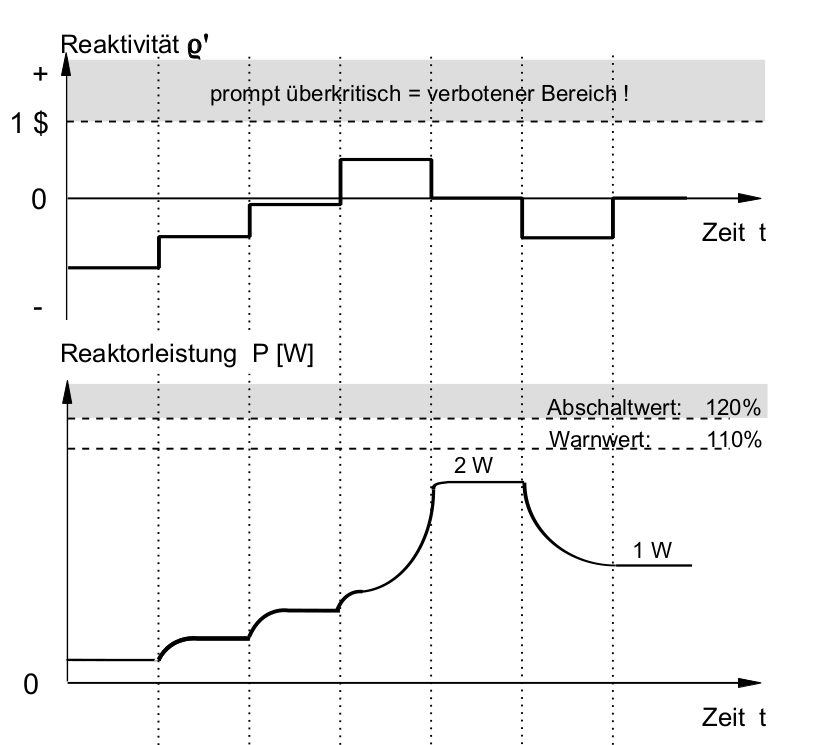
\includegraphics[scale=0.3]{pic/verhalten.png}
        \caption{Schematisches Verhalten bei Leistungseinstellung durch Steuerstabverschiebung}
        \label{skizze_leistung}
    \end{figure}
    Als abschließende Steuerstabpositionen erhält man $x_{1\unit{W}} = 2238$ und $x_{2\unit{W}} = 2250$ bei einer konstanten Temperatur von 22,4\unit{°C}. Dies scheint verhältnismäßig konstant und mit der Temperatur des Moderators korreliert zu sein.
    Die dosimetrischen Messungen werden an den Standorten gemäß Abbildung \ref{skizze} vorgenommen und notiert. Bei den in Tabelle \ref{dft:dosi} angegebenen Abständen (geklammerte Werte in Spalte \glqq Ort \grqq) handelt es sich um grobe Schätzwerte. \\ \ \\
         \begin{tabular}{l|c|c|c|c}
                \textbf{Ort} & \multicolumn{2}{c|}{\textbf{bei 1\unit{W}}} & \multicolumn{2}{c}{\textbf{bei 2\unit{W}}} \\
                \hline       & $\dot D_\gamma$ [\textit{$\frac{\mu Sv}{h}$}] & $\dot D_n$ [\textit{$\frac{\mu Sv}{h}$}]& $\dot D_\gamma$ [\textit{$\frac{\mu Sv}{h}$}]& $\dot D_n$ [\textit{$\frac{\mu Sv}{h}$}]\\
                \hline   Reaktortankwand ($\approx \unit[0]{m}$) & 12 & 2,5 & 27,5 & 4,3 \\
                Operatortisch ($\approx \unit[3]{m}$) & 1,4 & 0,2 & 2,5 & 0,6 \\
                Ecke ($\approx \unit[6]{m}$) & 0,6 & 0,14 & 0,5 & 0,13 
         \end{tabular}
         \captionof{table}{Dosimetrische Messung von Neutronen und Photonen an verschiedenen Orten und mit unterschiedlichen Leistungen}
         \label{dft:dosi}
         \ \\
    Dies hat Einfluss auf die getätigten Fits in Abbildung \ref{df:neu_abstand}, welche das Abstandsquadratgesetz für Neutronenstrahlung zeigen soll. Während sich die Dosisleistung bei einer Reaktorleistung von 1\unit{W} bei diesem Schätzwert sehr gut dem Abstandsquadratgesetz anpasst, weicht der Fit bei 2\unit{W} stärker ab. 
    Die zugrundeliegende Formel, die für die Fits verwendet wurde lautet wie folgt:
    \begin{equation*}
        \dot D_P = \frac{c_P}{\left(r_{Tank} + d\right)^2}
    \end{equation*}
    Dabei stellt $P$ die thermische Reaktorleistung dar, $r_Tank$ ist der Tankradius, $d$ der Abstand zum Tank undd $c_P$ ist eine Proportionalitätskonstante. Der Tankradius ist als $r_Tank = 1\unit{m}$ angenommen worden.
    Aufgrund dieses Fits ergeben sich folgende Proportionalitätskonstanten:
    $$ c_{1W} = (4,3 \pm 0,2)\unit{\frac{\mu Sv m^2}{h}} \ , \ c_{2W} = (2,5 \pm 0,07)\unit{\frac{\mu Sv m^2}{h}} $$
    \begin{figure}
        \centering
        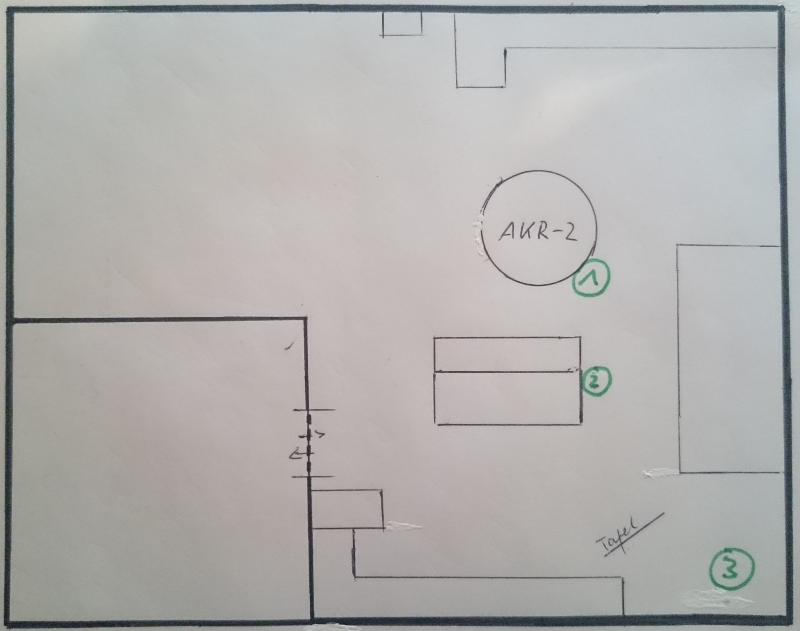
\includegraphics[scale=0.4]{pic/skizze_grundriss}
        \caption{Skizze des Grundrisses des Reaktorstandortes (nicht maßstabsgerecht); 1: Reaktorwand, 2:Operatortisch, 3: Ecke}
        \label{skizze}
    \end{figure}
        \begin{figure}
               \centering
               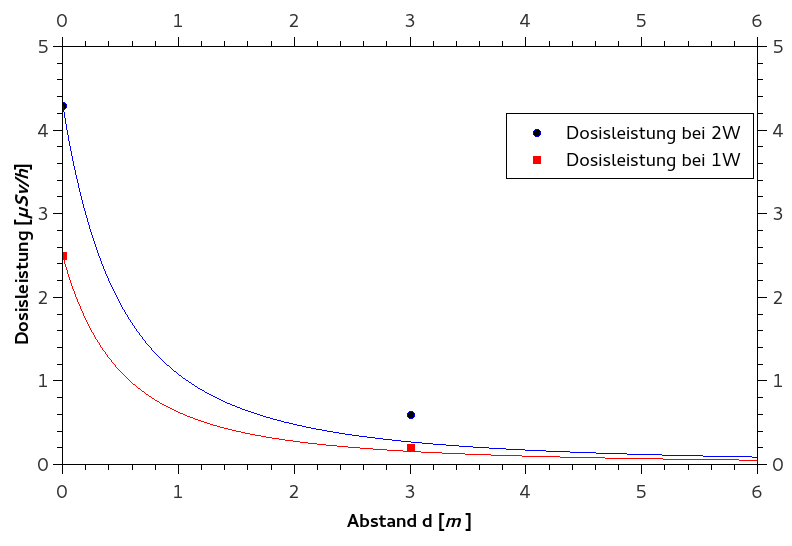
\includegraphics[scale=0.5]{pic/Neutronendosisleistung_Abstand}
               \caption{Dosisleistung der Neutronenstrahlung an verschiedenen Orten bei unterschiedlichen thermischen Leistungen}
               \label{df:neu_abstand}
        \end{figure}
    Die Fehler sind eine Ausgabe des Tools qtiplot und fallen durch die Abschätzung der Abstände in Wahrheit größer aus. Als Lehre hieraus kann direkt erschlossen werden, dass die Abstände genau zu notieren sind.
    Dennoch kann man den quadratischen Abfall mit Zunahme des Abstandes erkennen.
        \begin{figure}
            \subfigure[Dosisleistung von Neutronen\label{p:dosi_neu}]{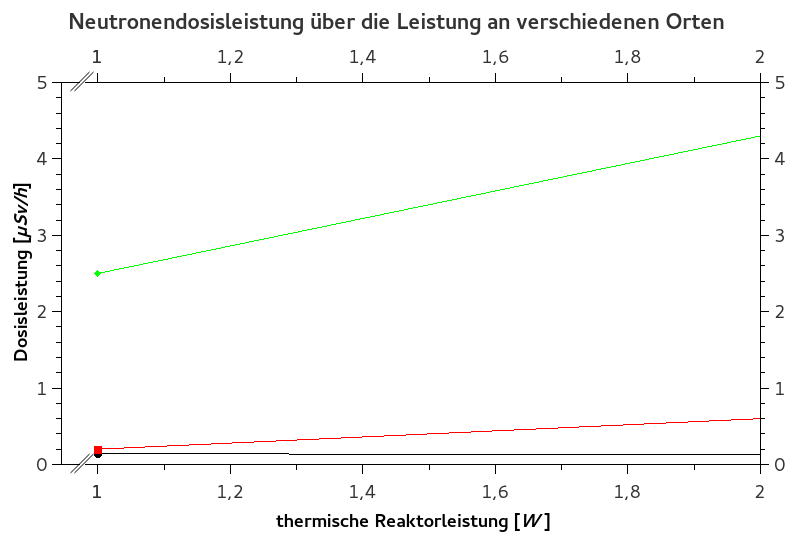
\includegraphics[scale=0.35]{pic/neutronendosisleistung}}
            \subfigure[$\gamma$-Dosisleistung\label{p:dosi_gamma}]{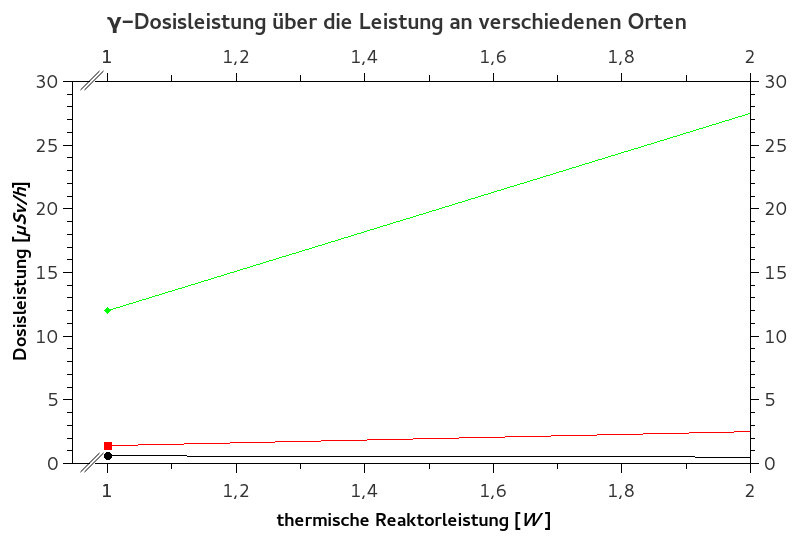
\includegraphics[scale=0.35]{pic/gamma_dosisleistung}}
            \caption{Dosisleistungen bei verschiedenen Reaktorleistungen}
            \label{df:dosi_g_n}                    
        \end{figure}
    Als nächstes wird die Zunahme der Dosisleistung von $\gamma$- und Neutronenstrahlung betrachtet. Für Neutronenstrahlung ist dies in Abbildung \ref{p:dosi_neu}, für $\gamma$-Strahlung in Abbildung \ref{p:dosi_gamma} dargestellt.
    Es ist deutlich sichtbar, dass die Dosisleistung mit Verdopplung der Reaktorleistung steigt. Weiterhin sieht man gut, dass mehr $\gamma$- als Neutronenstrahlung den Tank verlässt, was zu erwarten ist, da die Neutronen massiv sind und mit der Materie stärker interagieren können, wobei natürlich ebenfalls Strahlung frei wird.
    Weiterhin wird der Anstieg der Dosisleistung bei zunehmender Entfernung deutlich kleiner. Dies ist aufgrund des Abstandsquadratgesetzes ohnehin zu erwarten.
    Ebenfalls sichtbar wird in Abbildung \ref{df:dosi_g_n} ein kleiner Abfall der Dosisleistung in der Ecke. Dies betrifft beide vermessenen Strahlungsarten. Es kann sich hierbei um Messfehler handeln, oder um eine Art Sättigungsphänomen.
    
    \ \\    


    \subsection{Steuerstabkalibrierung}

